\section[Designing Questions]{design}

\begin{frame}
  \frametitle{Disclaimer}
  Some examples are inspired by Greg Wilsons book
 \begin{center}
  \sf{Teaching Tech Together} (CRC Press, 2020)
 \end{center}
 Some ideas are based on own experience, some on other sources.
\end{frame}

\subsection{Question Types}

\begin{frame}
  \frametitle{Purposes \ldots}
  Before diving into Question Design, note:
  \begin{itemize}
    \item a question can be asked with a certain aim
    \item different courses ask for different knowledge / skills
    \item $\curvearrowright$ questions need to be designed and choosen with care
  \end{itemize}
\end{frame}

% overview
% background selection

\subsection{Multiple Choice Questions}

\begin{frame}
 \frametitle{Multiple Choice -- When?}

 Multiple Choice Questions (MCQs) are popular when designing e-learning tests \ldots\vspace{-1em}
 \pause
 \newline
 \only<2->{\question{When are they most suitable?}}
 \pause
 Suppose you are teaching children and you give them this MCQ:
 \exercise[Testing Conceptions]{
  What is 37 + 15?
  \begin{enumerate}[a)]
   \item 52  {\color{pdarkgrey}correct}
   \item 42  {\color{pdarkgrey}child did not understand ``carrying''}
   \item 412 {\color{pdarkgrey}child treated every column seperately}
   \item 43  {\color{pdarkgrey}knows she has to carry 1, but to wrong column}
  \end{enumerate}
 }
\end{frame}


\begin{frame}
 \frametitle{Multiple Choice -- When? (continued)}
 
 The Young-Child question rephrased for newbies to the SLURM batch system:
 \vspace{-1em}
 \exercise[Testing Conceptions about SLURM]{
   Think of a cluster with 20 core nodes. If a job is submitted with the following parameterisation, how many nodes are reserved?\newline
   \texttt{\#SBATCH -n 20}\newline
   \texttt{\#SBATCH -c 2}
   \begin{enumerate}[a)]
    \item 2 {\color{pdarkgrey}correct}
    \item 4 {\color{pdarkgrey}user did correctly multiply, but is not aware of the 20 cores}
    \item 1 {\color{pdarkgrey}user did not multiply by \texttt{-c 2}}
    \item unkown without \texttt{N}-flag {\color{pdarkgrey}user did not understand the concept}
   \end{enumerate}
  }
\end{frame}

\begin{frame}
  \frametitle{What is in the Arsenal?}
  \begin{columns}
   \begin{column}{.5\textwidth}
    MCQs aren't everything:
     \begin{enumerate}
      \item Freetext (if short and explicit)
      \item Filling in blanks (for code; to be implemented)
      \item Parson Problem (can by done as MCQ; in a minute)
      \item Tracing (can by done as MCQ; in a minute)
     \end{enumerate}
   \end{column}
   \begin{column}{.5\textwidth}
       \centering
      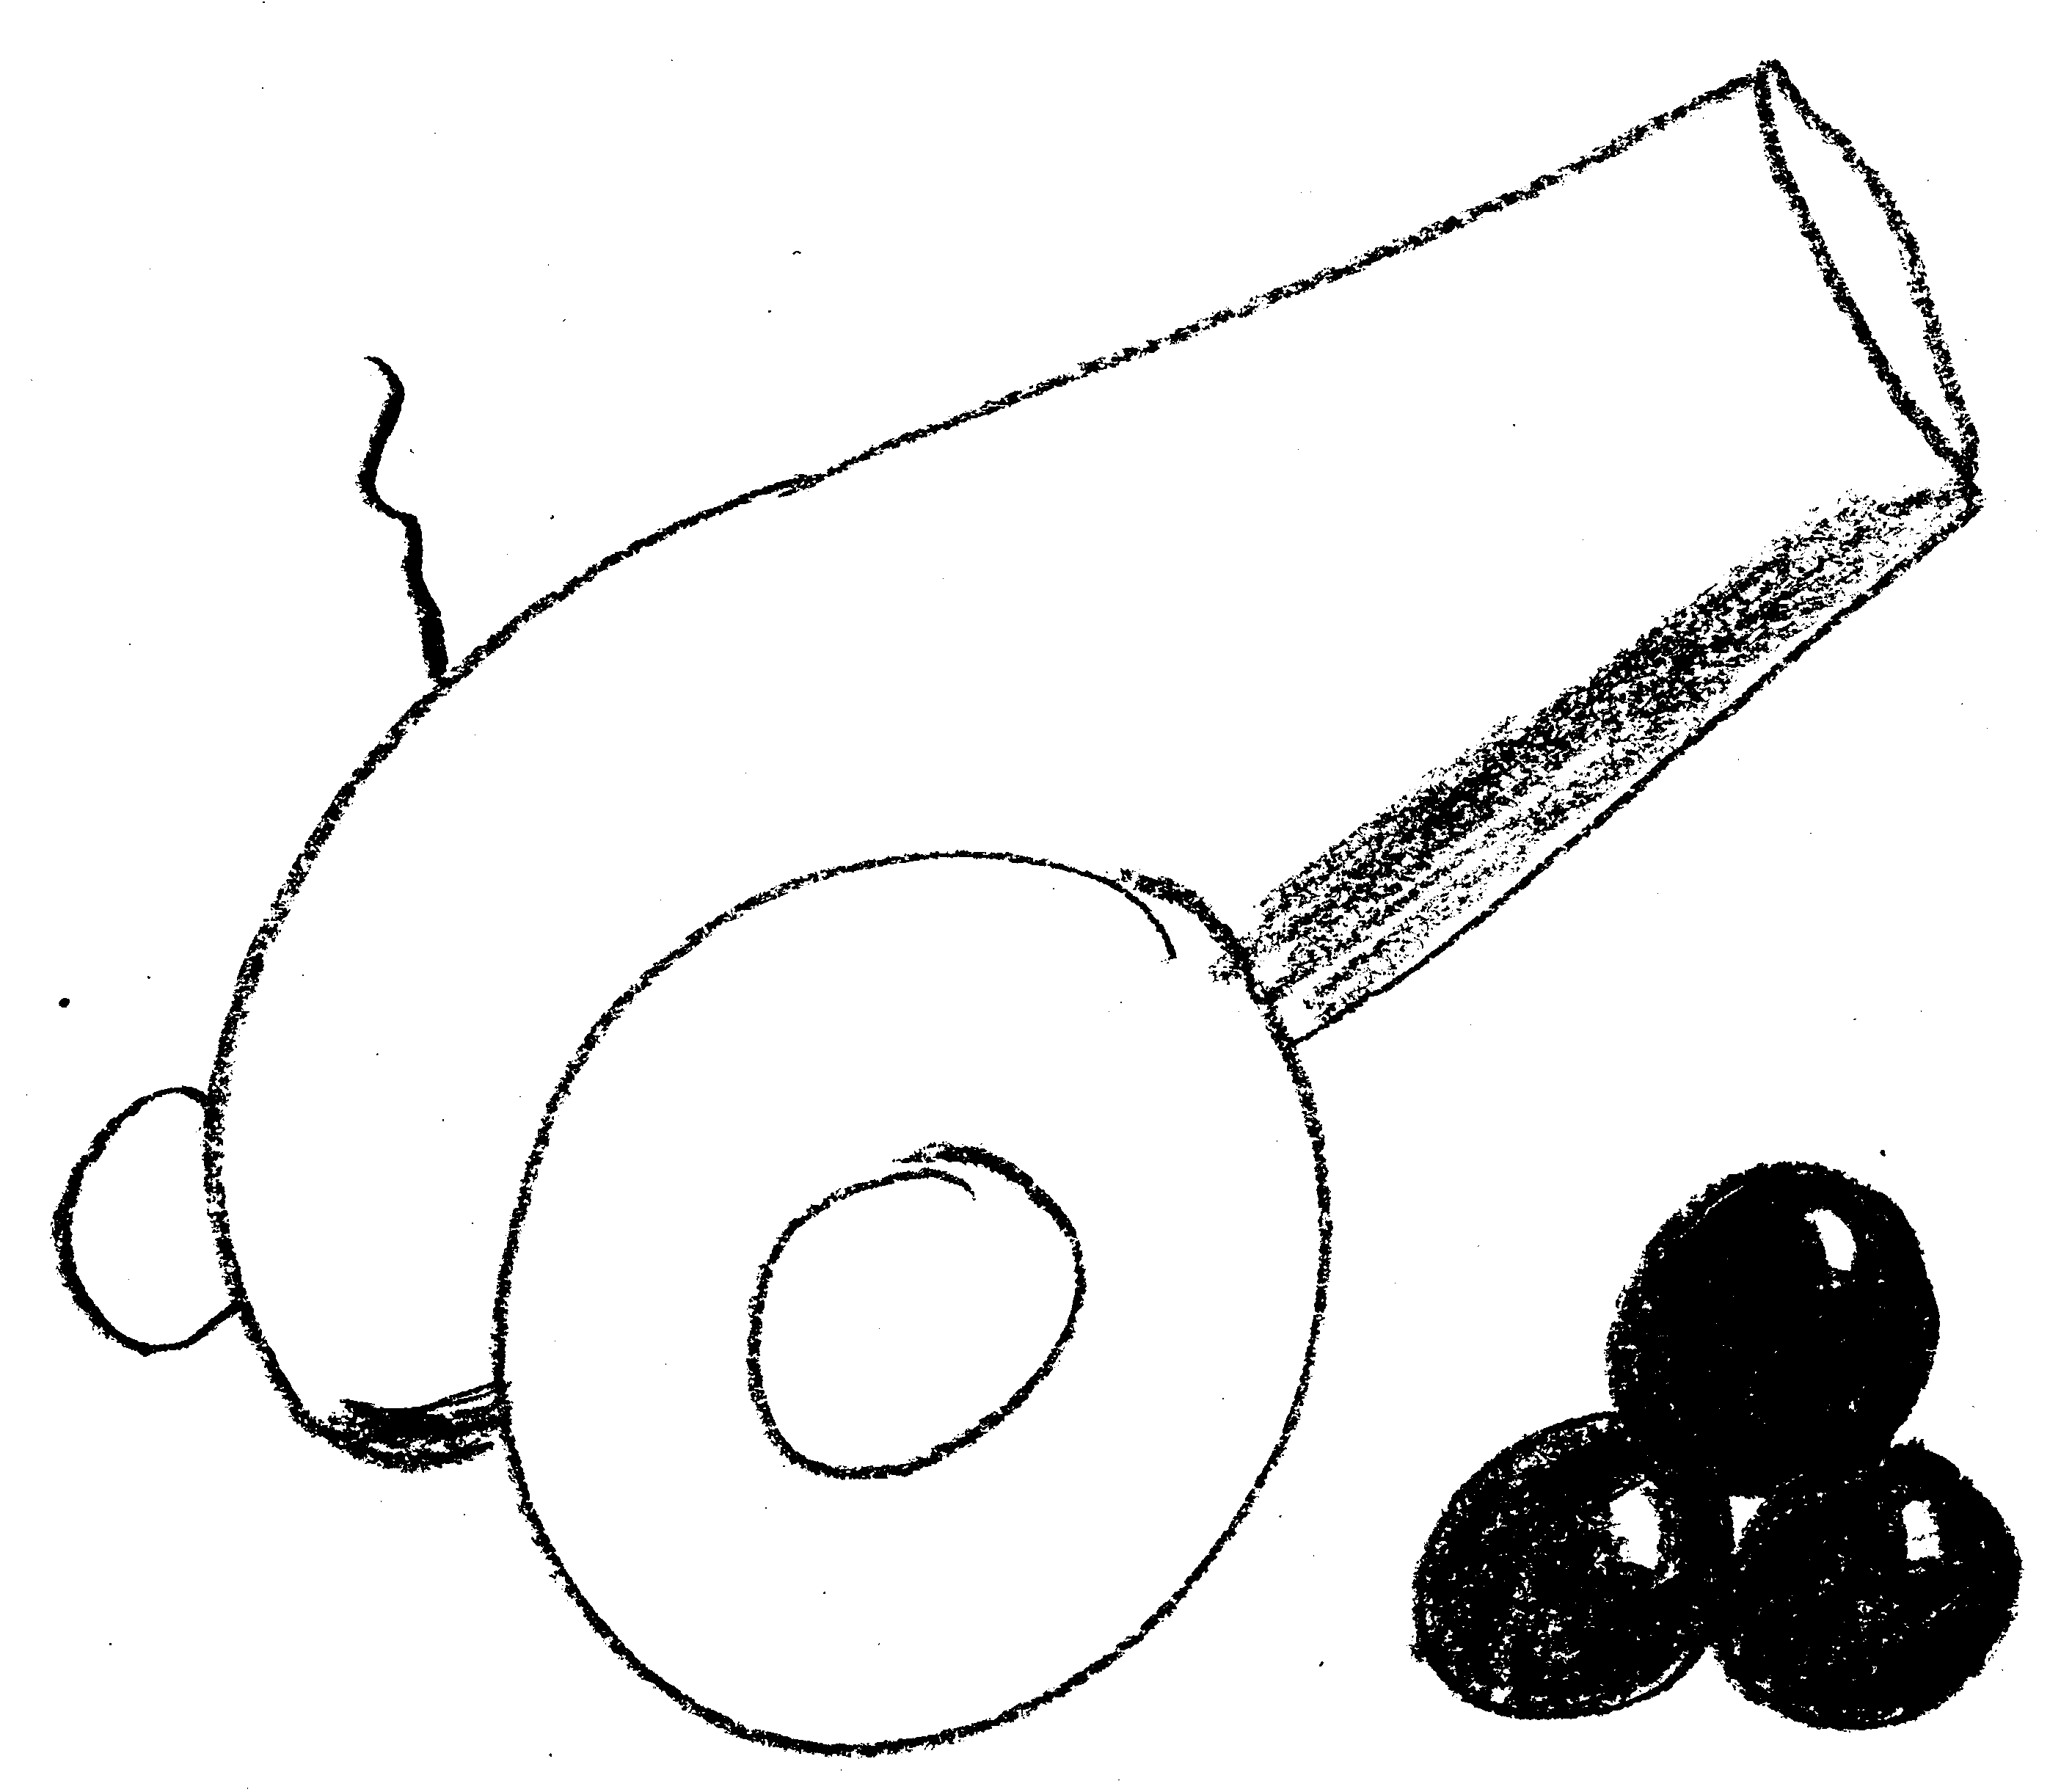
\includegraphics[width=0.6\textwidth]{images/arsenal}
    \end{column}
  \end{columns}
\end{frame}

\begin{frame}
  \frametitle{Fill in Blanks}
\end{frame}

\begin{frame}
  \frametitle{Parson Problems}
\end{frame}

\begin{frame}
  \frametitle{Tracing}
\end{frame}

\begin{frame}
  \frametitle{Points}
\end{frame}
